\documentclass[10pt]{beamer}

\usepackage{ucs}
\usepackage[spanish]{babel}
\usepackage[utf8x]{inputenc}

\usepackage{amsmath,amsfonts,,amssymb,latexsym}


%------- Paquetes hiperreferencias------------%
\usepackage{hyperref}

%------- Paquetes glosarios-------------------%
\usepackage[acronym]{glossaries}
\makeglossaries

%------- Insertar archivos .gif---------------%
\usepackage{graphicx}
\usepackage{epstopdf}

\epstopdfDeclareGraphicsRule{.gif}{png}{.png}{%
  convert gif:#1 png:\OutputFile
}
\AppendGraphicsExtensions{.gif}


\title{Instrument Landing System}
\author{Ing. Jorge Garc\'ia (jgarcia@efn.uncor.edu)}
\date{\today}


\begin{document}
\maketitle

\begin{frame}
  El Instrument Landing System (ILS) es un sistema para guía de precisión que los pilotos utilizan para efectuar aproximaciones y aterrizajes de precisión en una pista en condiciones de vuelo por Instrumentos (IFR - Instrument Flight Rules) cuando las condiciones atmosféricas así lo exigen (IMC - Instrument Meteorological Conditions).

\begin{center}
  
\includegraphics[width=0.8\textwidth]{imagenes/tablero.eps}
\end{center}

\end{frame}

\begin{frame}
  Un ILS consiste de dos subsistemas independientes: uno sirve para proporcionar guía lateral (localizer) y el otro para proporcionar guía vertical (glide slope).

  \begin{center}
    \includegraphics[width=0.7\textwidth]{imagenes/ils-system.gif}
  \end{center}

\end{frame}

\begin{frame}
Una serie de antenas localizadoras (LOC o localizer) están situadas normalmente a unos 1000 pies (305 m) del final de la pista y suelen consistir en 8 ó 14 antenas direccionales. Se transmiten señales portadoras entre los 108 MHz y 112MHz definidas para cada localizador. Estas portadoras se modulan con 90 Hz y 150 Hz y con distintas fases .

\begin{center}
  
\includegraphics[width=0.8\textwidth]{imagenes/Whiteman_localizer.eps}

   {\small Disposición del localizador y luces de
    aproximación en la base de la USAF Whiteman, Johnson County,
    Missouri.}
\end{center}

\end{frame}

\begin{frame}
  Esto produce el efecto que la señal de 150 Hz predomine en el lado derecho de pista y la de 90 Hz en el izquierdo. El receptor del localizador en el avión mide la diferencia entre la modulación entre las señales de 90 Hz y 150 Hz: cuando la diferencia es de cero, la antena receptora está en la línea central del localizador, lo que normalmente coincide con el centro de la pista.


\begin{center}
  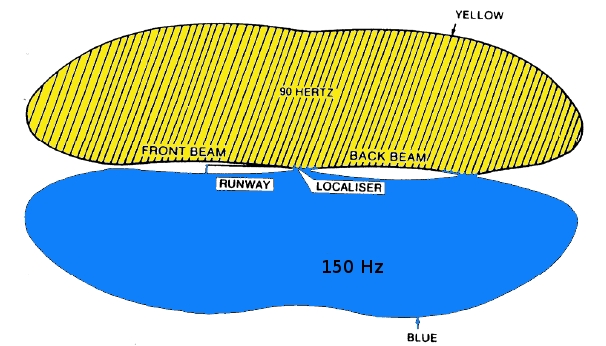
\includegraphics[width=0.8\textwidth]{imagenes/localizer-color.jpg}

\end{center}

\end{frame}

\begin{frame}
  Una antena transmisora de la senda de planeo (GS, del inglés: glideslope) se sitúa a un lado de la zona de la pista donde se produce la toma. La señal GS se transmite a una frecuencia de entre 328,6 MHz y 335,4 MHz, usando una técnica similar a la del localizador; la señal está situada para marcar una senda de planeo de aproximadamente 3º sobre la horizontal.

\begin{center}
  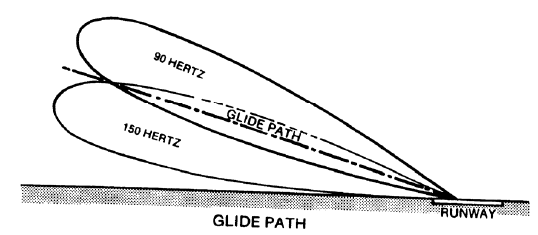
\includegraphics[height=2.6cm]{imagenes/glidepath.jpg} \hspace{3mm}
  \includegraphics[height=2.6cm]{imagenes/antena-GS.eps}
\end{center}

\end{frame}

\begin{frame}
  Las frecuencias del localizador y la senda de planeo están emparejadas de manera que sólo se requiere seleccionar una frecuencia para sintonizar ambos receptores. El localizador proporciona una señal de código morse transmitida a 1020 Hz para permitir la identificación. Por ejemplo, en el aeropuerto de Barajas, se transmitiría MAA para la pista 33L. Esto permite saber si el ILS está operando con normalidad o si está correctamente sintonizado. La señal de senda de planeo no transmite ninguna señal de identificación, por lo que solo se depende del localizador.


\end{frame}


\begin{frame}
Las radiobalizas operan a 75 MHz y se utilizan para indicar la altura y posición aproximadas a las que se encuentra el avión durante su aproximación.


  \begin{columns}
    \begin{column}{0.5\textwidth}{\tiny
 \begin{itemize}
      \item {\bf Radiobaliza exterior (OM, del inglés: outer marker):} localizada a 3,9 millas náuticas (7,2 km) del umbral de la pista. Emite dos rayas (morse) por segundo con un tono de 400 Hz; su indicador es azul. Se utiliza esta radiobaliza para ayudar a los chequeos de altura, distancia y funcionamiento del equipamiento. Se puede combinar con un NDB para crear una Radiobaliza Exterior de Localizador (LOM, del inglés: Locator Outer Marker).
	 \item \textbf{Radiobaliza intermedia (MM, del inglés: middle marker): }se localiza para que, en condiciones de baja visibilidad informe que el contacto con la pista es inminente. Está modulada con un tono de 1300 Hz y emite puntos y rayas (morse) alternativos. Su color es ámbar.
	 \item \textbf{Radiobaliza interior (IM, del inglés: inner marker):} cuando está instalada, se localiza para que en condiciones de baja visibilidad se indique que se está a punto de cruzar el umbral de la pista. En esta posición un avión normalmente llega a las condiciones mínimas de la Categoría II. La modulación es de puntos a 3000 Hz, 6 por segundo. Su color es blanco.
    \end{itemize}
}
    \end{column}
    \begin{column}{0.5\textwidth}
    \includegraphics[width=\textwidth]{imagenes/markers.gif}

    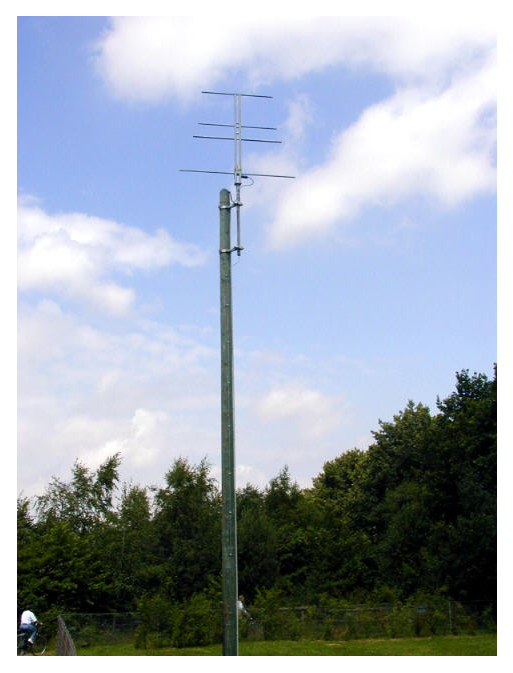
\includegraphics[height=2.5cm]{imagenes/antena-radiobaliza.eps}
  \end{column}

  \end{columns}

\end{frame}

\end{document}

